\section{Spring Problems I}

\noindent
We consider the motion of an object of mass $m$, suspended from a
spring of negligible mass. We say that the spring--mass system is
in {\color{blue}\it  equilibrium\/} when the object is at rest and the forces
acting on it sum to zero. The position of the object in this case is
the {\color{blue}\it equilibrium position\/}. We define $y$ to be the displacement
of the object from its equilibrium position (Figure~\ref{figure:6.1.1}),
measured positive upward.

\begin{figure}[htbp]
\color{blue}
  \begin{minipage}[b]{0.5\linewidth}
    \centering
   \scalebox{.6}{
  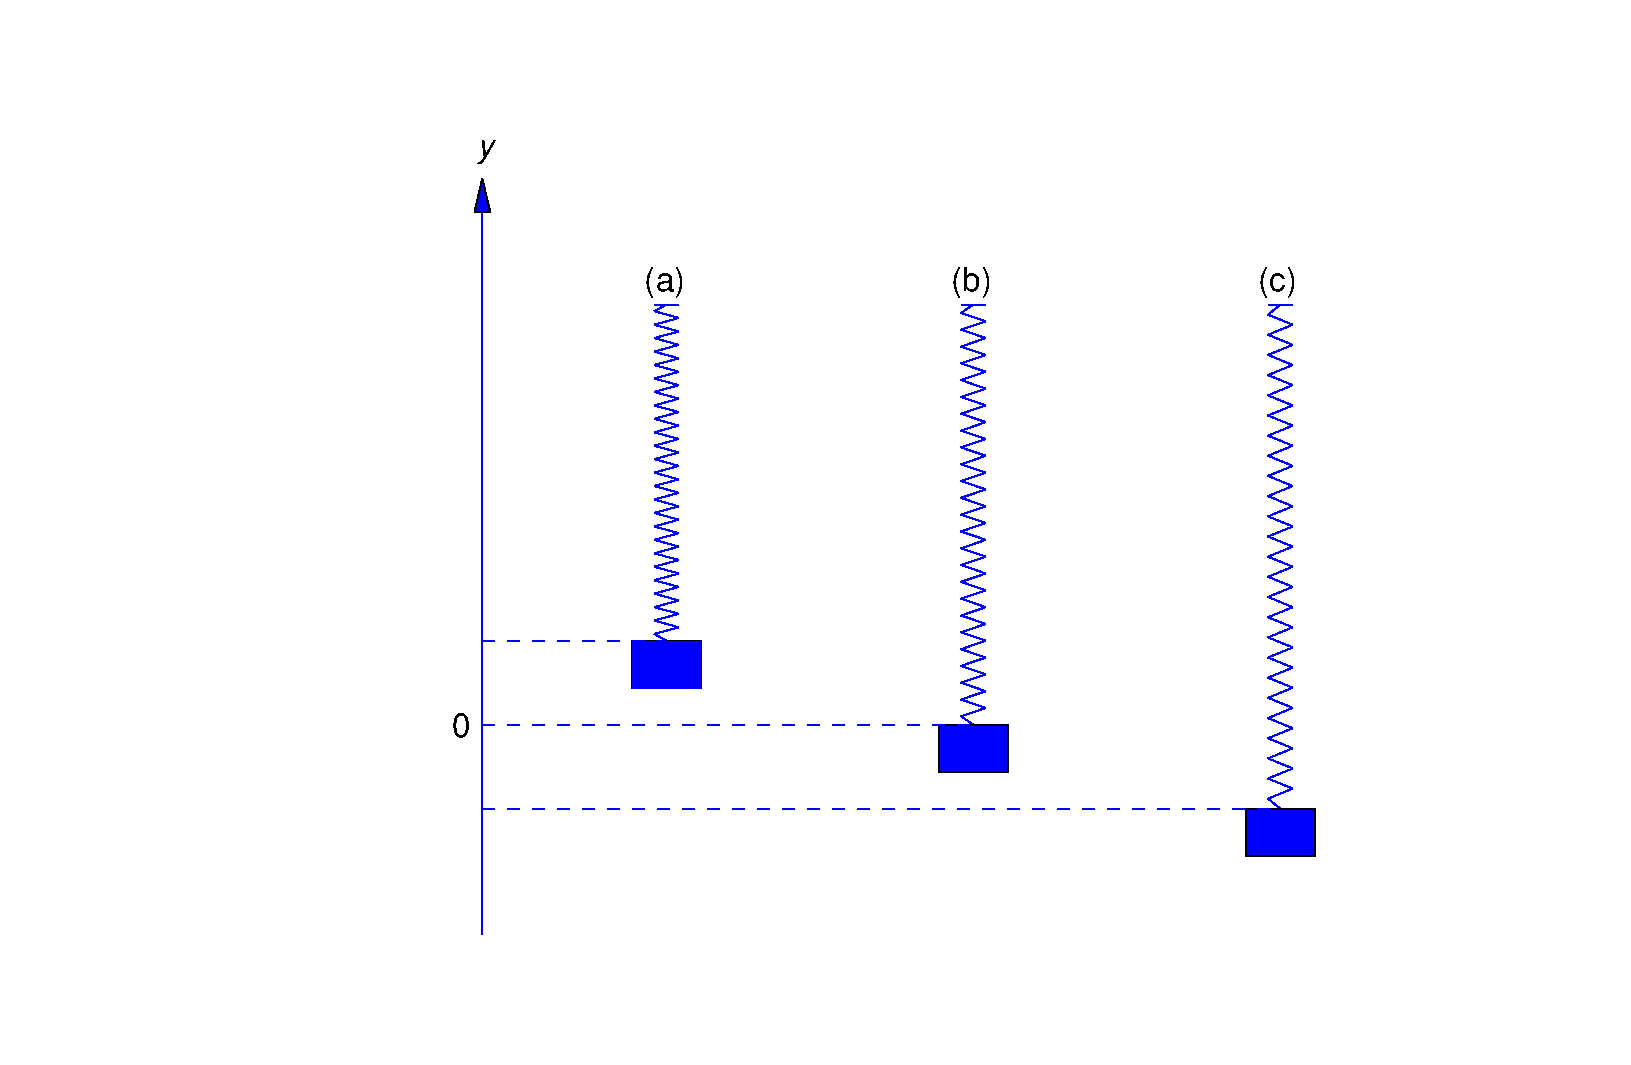
\includegraphics[bb=-78 148 689 643,width=5.67in,height=3.66in,keepaspectratio]{fig060101}}
\caption{ { \bf (a)}  $y>0$ \,  {\bf (b)} $y=0$,  \,    {\bf (c)}  $y<0$}
  \label{figure:6.1.1}
\end{minipage}
  \begin{minipage}[b]{0.5\linewidth}
    \centering
   \scalebox{.7}{
  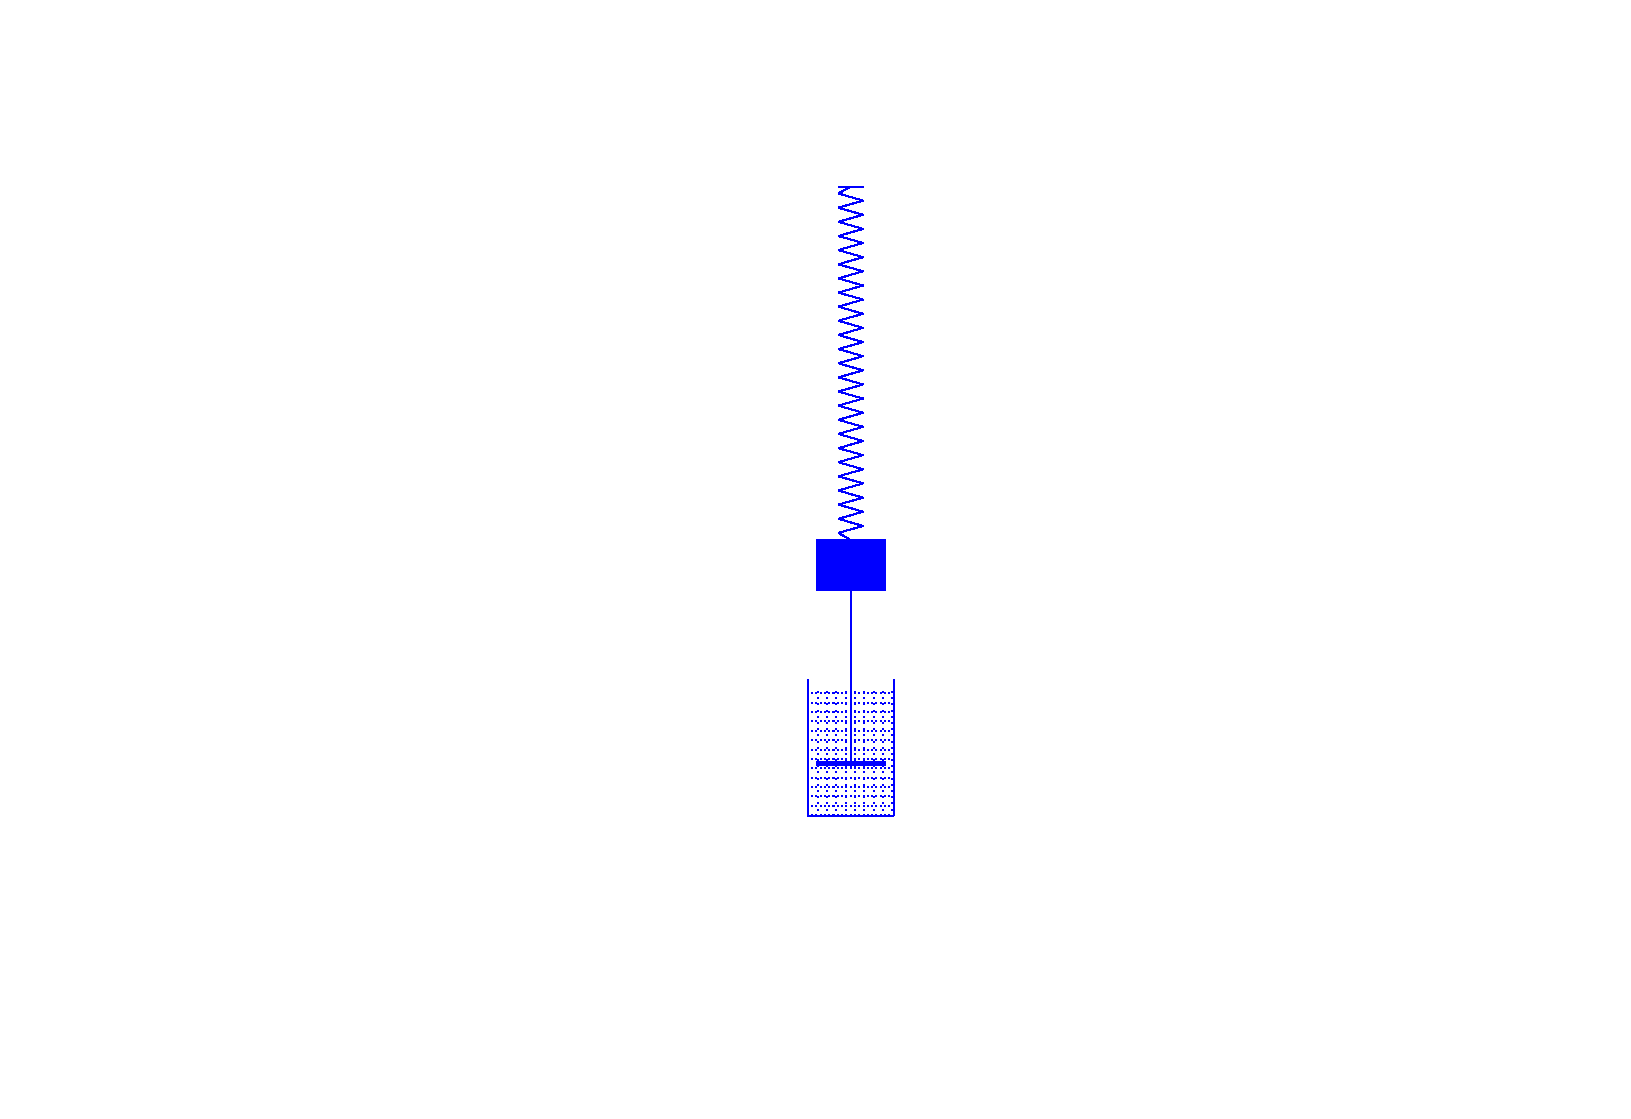
\includegraphics[bb=-78 135 689 656,width=5.67in,height=3.85in,keepaspectratio]{fig060102} }
\caption{ A spring -- mass system with damping}
  \label{figure:6.1.2}
\end{minipage}
\end{figure}

Our model accounts for the following kinds of forces acting on the
object:

\begin{itemize}
\item The force $-mg$, due to gravity.

\item A force $F_{s}$ exerted by the spring resisting change in its
length. The {\color{blue}\it natural length} of the spring is its length with
no mass attached. We assume that the spring obeys
\href{https://mathshistory.st-andrews.ac.uk/Biographies/Hooke/}
{\color{blue}\it Hooke's law}:
If the length of the spring is changed by an amount $\Delta L$
from its natural length,  then the spring exerts a force $F_{s}=k\Delta
L$, where $k$ is a positive number called the {\color{blue}\it spring constant\/}.
If the spring is stretched then  $\Delta L>0$ and $F_{s}>0$, so the
spring force is upward, while if the spring is compressed then $\Delta
L<0$ and $F_{s}<0$, so the spring force is downward.

\item A {\color{blue}\it damping force\/} $F_{d}=-cy'$ that resists the motion with
a force proportional to the velocity of the object. It may be due to
air resistance or friction in the spring. However, a convenient way to
visualize a damping force is to assume that the object is rigidly
attached to a piston with negligible mass immersed in a cylinder
(called a {\color{blue}\it dashpot\/}) filled with a viscous liquid
(Figure~\ref{figure:6.1.2}). As the piston moves, the liquid exerts a
damping force. We say that the motion is {\color{blue}\it undamped\/} if $c=0$, or
{\color{blue}\it damped\/} if $c>0$.

\item An external force $F$, other than the force due to gravity, that
may vary with $t$, but is independent of displacement and velocity. We
say that the motion is {\color{blue}\it free\/} if $F\equiv0$, or {\color{blue}\it forced\/}
if $F\not\equiv0$.

\end{itemize}

From Newton's second law of motion,
\begin{equation}\label{eq:6.1.1}
my''=-mg+F_{d}+F_{s}+F=-mg-cy'+F_{s}+F.
\end{equation}
We must now relate $F_{s}$ to $y$. In the absence of external forces the
object stretches the spring by an amount $\Delta l$ to assume its
equilibrium position (Figure~\ref{figure:6.1.3}). Since the sum of the forces acting on the object
is then zero, Hooke's Law implies that $mg=k\Delta l$. If the object
is displaced $y$ units from its equilibrium position, the total
change in the length of the spring is $\Delta L=\Delta l-y$,
 so Hooke's law implies that
 $$
F_{s}=k\Delta L=k\Delta l-ky.
$$
Substituting this into \eqref{eq:6.1.1} yields
$$
my''=-mg-cy'+k\Delta L-ky+F.
$$
Since $mg=k\Delta l$ this can be written as
\begin{equation}\label{eq:6.1.2}
my''+cy'+ky=F.
\end{equation}
We call this {\color{blue}\it the equation of motion\/}.

\begin{figure}[tbp]
  \centering
  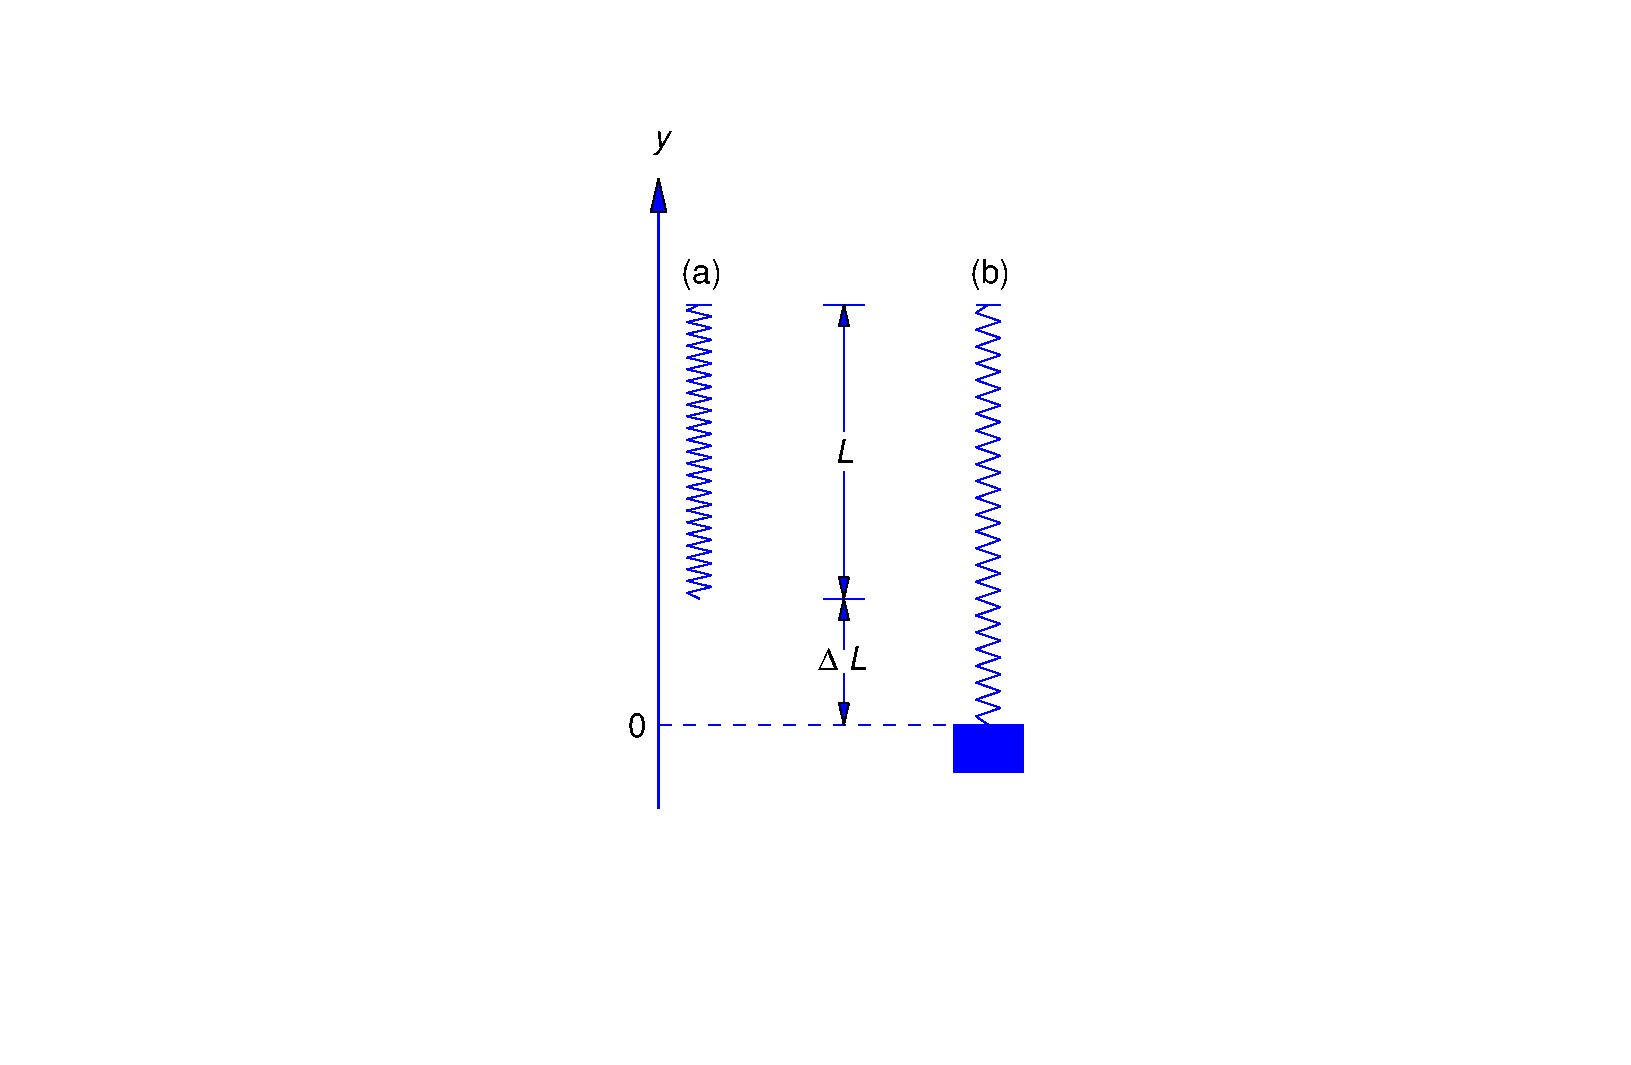
\includegraphics[bb=-78 148 689 643,width=5.67in,height=3.66in,keepaspectratio]{fig060103}
\color{blue}
\caption{ {\bf(a)} Natural length of spring  \,
{\bf (b)} Spring stretched by mass}
  \label{figure:6.1.3}
\end{figure}

\boxit{Simple Harmonic Motion}

\noindent
Throughout the rest of this section we'll consider spring--mass
systems without damping; that is, $c=0$. We'll consider systems with
damping in the next section.

We first consider the case where the motion is also free; that is,
$F$=0. We begin with an example.

\begin{example}\label{example:6.1.1}\rm
An object stretches a spring 6 inches in equilibrium.
\begin{alist}
\item % (a)
Set up the equation of motion and find its general solution.

\item % (b)
Find the displacement of the object for $t>0$ if it's initially
displaced 18 inches above equilibrium and given a downward velocity of
3 ft/s.
\end{alist}
\end{example}

\solutionpart{a}
Setting $c=0$ and $F=0$ in \eqref{eq:6.1.2} yields the equation of motion
$$
my''+ky=0,
$$
which we rewrite as
\begin{equation}\label{eq:6.1.3}
y''+\frac{k}{m}y=0.
\end{equation}
Although we would need the weight of the object to obtain $k$ from the
equation $mg=k\Delta l$ we can obtain $k/m$ from $\Delta l$ alone;
thus, $k/m=g/\Delta l$. Consistent with the units used in the problem
statement, we take $g=32$ ft/s$^{2}$. Although $\Delta l$ is stated in
inches, we must convert it to feet to be consistent with this choice
of $g$; that is, $\Delta l=1/2$ ft. Therefore
$$
\frac{k}{m}=\frac{32}{1/2}=64
$$
and \eqref{eq:6.1.3} becomes
\begin{equation}\label{eq:6.1.4}
y''+64y=0.
\end{equation}
 The characteristic equation of \eqref{eq:6.1.4} is
$$
r^{2}+64=0,
$$
which has the zeros $r=\pm8i$. Therefore the general solution of
\eqref{eq:6.1.4} is
\begin{equation}\label{eq:6.1.5}
y=c_{1}\cos8t+c_{2}\sin8t.
\end{equation}

\solutionpart{b}
The initial upward displacement of 18 inches is positive and must be
expressed in feet. The initial downward velocity is negative;   thus,
$$
y(0)=\frac{3}{2}\mbox{\quad and \quad}y'(0)=-3.
$$
 Differentiating \eqref{eq:6.1.5} yields
\begin{equation}\label{eq:6.1.6}
y'=-8c_{1}\sin8t+8c_{2}\cos8t.
\end{equation}
Setting $t=0$ in \eqref{eq:6.1.5} and \eqref{eq:6.1.6} and imposing the
initial conditions shows that $c_{1}=3/2$ and $c_{2}=-3/8$. Therefore
$$
y=\frac{3}{2}\cos8t-\frac{3}{8}\sin8t,
$$
where $y$ is in feet (Figure~\ref{figure:6.1.4}).

\begin{figure}[tbp]
  \centering
  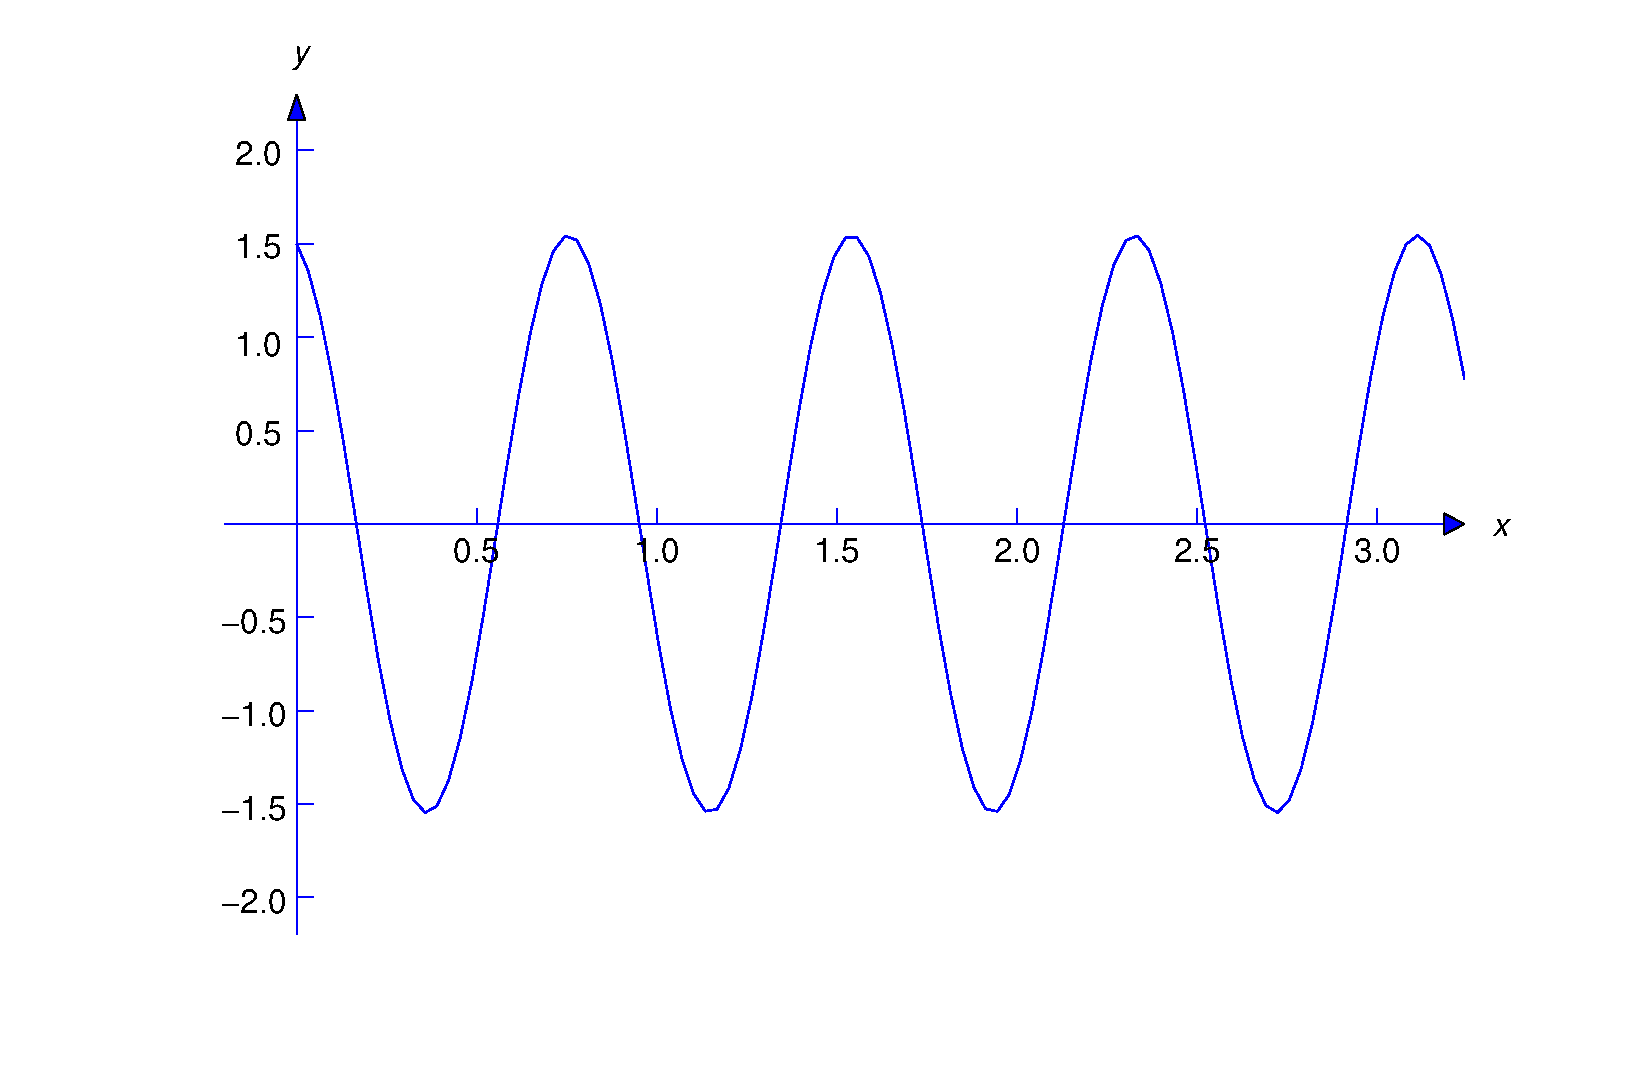
\includegraphics[bb=-78 148 689 643,width=5.67in,height=3.66in,keepaspectratio]{fig060104}
\color{blue}
\caption{$y=\dst{}{\frac{3}{2}}\cos8t-\frac{3}{8}\sin8t$}
  \label{figure:6.1.4}
\end{figure}

We'll now consider the equation
$$
my''+ky=0
$$
where $m$ and $k$ are arbitrary positive numbers. Dividing through by
$m$ and defining $\omega_{0}=\sqrt{k/m}$ yields
$$
y''+\omega_{0}^{2}y=0.
$$
The general solution of this equation is
\begin{equation}\label{eq:6.1.7}
y=c_{1}\cos\omega_{0}t+c_{2}\sin\omega_{0}t.
\end{equation}
We can rewrite this in a more useful form by defining
\begin{equation}\label{eq:6.1.8}
R=\sqrt{c_{1}^{2}+c_{2}^{2}},
\end{equation}
and
\begin{equation}\label{eq:6.1.9}
c_{1}=R\cos\phi\mbox{\quad and \quad}c_{2}=R\sin\phi.
\end{equation}
Substituting from \eqref{eq:6.1.9} into \eqref{eq:6.1.7} and applying the
identity
$$
\cos\omega_{0}t\cos\phi+\sin\omega_{0}t\sin\phi=\cos(\omega_{0}t-\phi)
$$
yields
\begin{equation}\label{eq:6.1.10}
y=R\cos(\omega_{0}t-\phi).
\end{equation}

From \eqref{eq:6.1.8} and \eqref{eq:6.1.9} we see that the $R$ and $\phi$
can be interpreted as polar coordinates of the point with rectangular
coordinates $(c_{1},c_{2})$ (Figure~\ref{figure:6.1.5}). Given $c_{1}$ and
$c_{2}$, we can compute $R$ from \eqref{eq:6.1.8}. From \eqref{eq:6.1.8} and
\eqref{eq:6.1.9}, we see that $\phi$ is related to $c_{1}$ and $c_{2}$ by
$$
\cos\phi=\frac{c_{1}}{\sqrt{c_{1}^{2}+c_{2}^{2}}}\mbox{\quad and \quad}\sin\phi=
\frac{c_{2}}{\sqrt{c_{1}^{2}+c_{2}^{2}}}.
$$
There are infinitely many angles $\phi$, differing
 by integer multiples of $2\pi$, that satisfy these equations. We
will always choose $\phi$ so that $-\pi\le\phi<\pi$.

\begin{figure}[tbp]
  \centering
  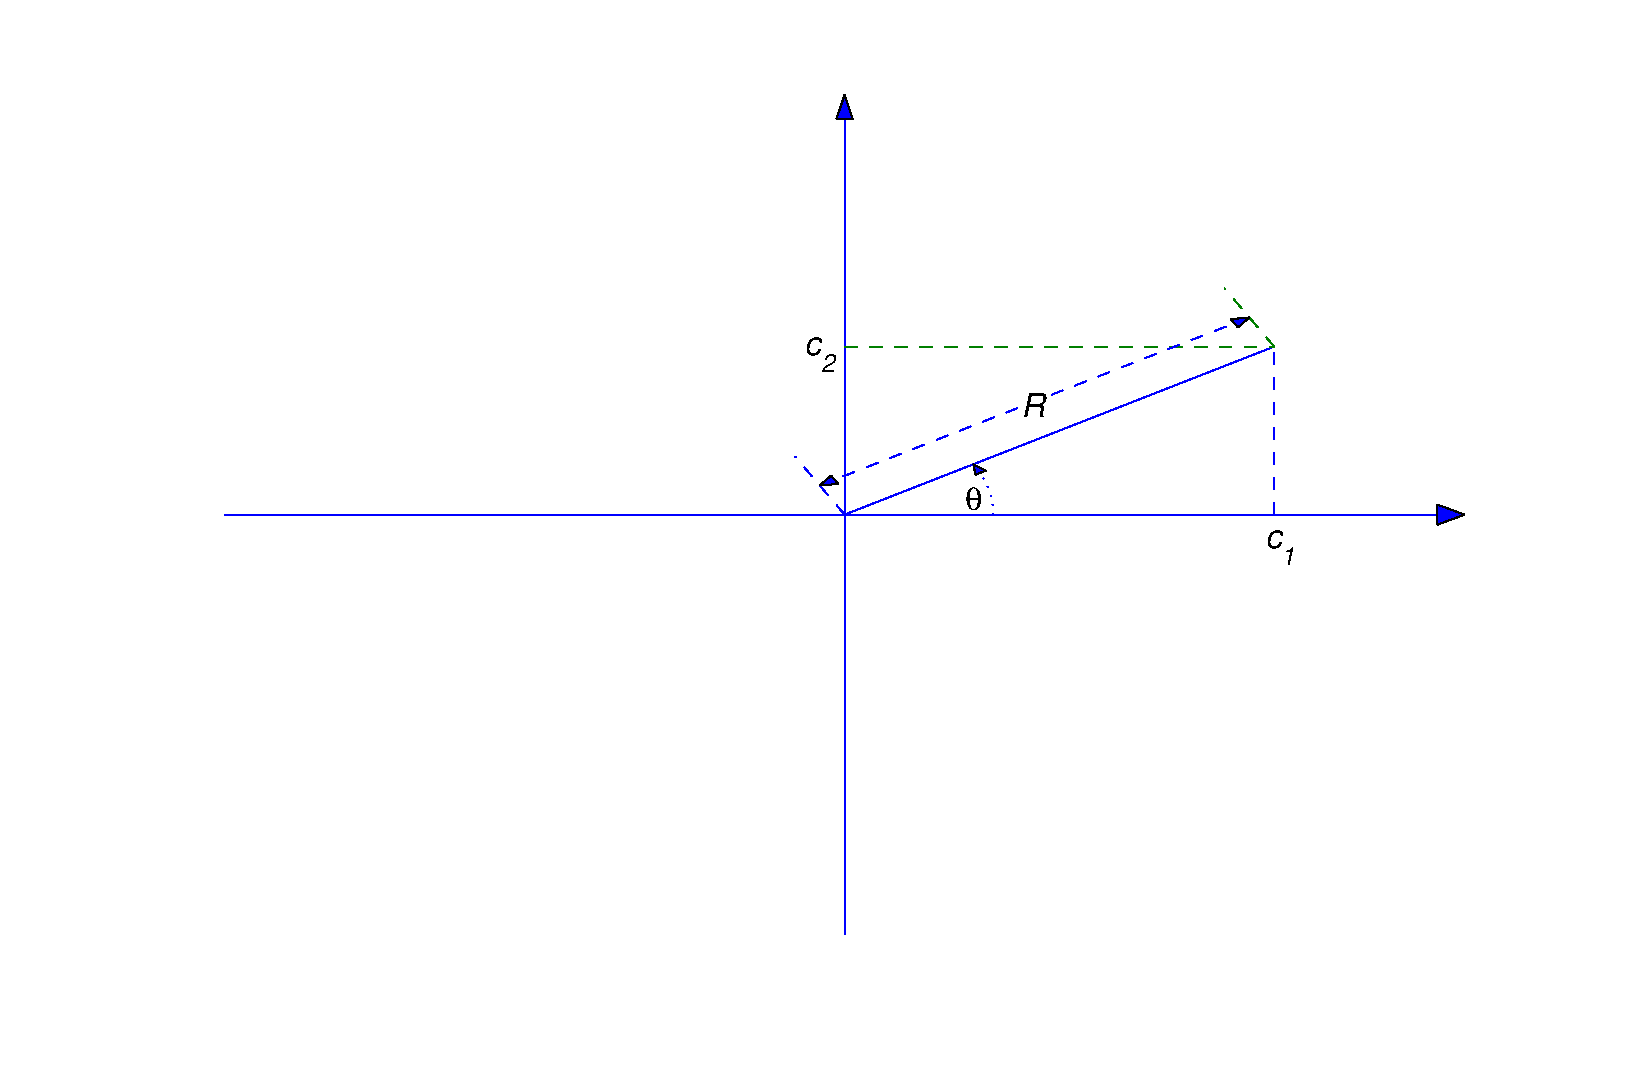
\includegraphics[bb=-78 148 689 643,width=5.67in,height=3.66in,keepaspectratio]{fig060105}
\color{blue}
\caption{$R=\protect\sqrt{c_{1}^{2}+c_{2}^{2}}$;  \quad
$c_{1}=R\cos\phi$;  \quad $c_{2}=R\sin\phi$}
  \label{figure:6.1.5}
\end{figure}

The motion described by \eqref{eq:6.1.7} or \eqref{eq:6.1.10}
is  {\color{blue}\it simple harmonic motion\/}. We see from either of these
equations that the motion is periodic, with period
$$
T=2\pi/\omega_{0}.
$$
This is the time required for the object to complete one full cycle of
oscillation (for example, to move from its highest position to its
lowest position and back to its highest position). Since the highest
and lowest positions of the object are $y=R$ and $y=-R$, we say that
$R$ is the {\color{blue}\it amplitude\/} of the oscillation. The angle $\phi$ in
\eqref{eq:6.1.10} is the {\color{blue}\it phase angle\/}. It's measured
in
radians. Equation~\eqref{eq:6.1.10} is the {\color{blue}\it amplitude--phase
form\/} of the displacement. If $t$ is in seconds then $\omega_{0}$ is
in radians per second (rad/s);   it's  the {\color{blue}\it
frequency\/} of
the motion. It is also called the {\color{blue}\it natural frequency\/} of
the spring--mass system without damping.

\begin{example}\label{example:6.1.2}\rm
We found the displacement of the object
 in Example~\ref{example:6.1.1} to be
$$
y=\frac{3}{2}\cos8t-\frac{3}{8}\sin8t.
$$
Find the frequency, period, amplitude, and phase angle of the motion.
\end{example}

\solution
The frequency is $\omega_{0}=8$ rad/s, and the period is
$T=2\pi/\omega_{0}=\pi/4$ s. Since $c_{1}=3/2$ and $c_{2}=-3/8$,
the amplitude is
$$
R=\sqrt{c^{2}_{1}+c^{2}_{2}}=\sqrt{\left(\frac{3}{2}\right)^{2}+\left(\frac{3}{8}\right)^{2}}
=\frac{3}{8}\sqrt{17}.
$$
The phase angle is determined by
\begin{equation}\label{eq:6.1.11}
\cos\phi=\frac{\frac{3}{2}}{{\frac{3}{8}}\sqrt{17}}=\frac{4}{\sqrt{17}}
\end{equation}
and
\begin{equation}\label{eq:6.1.12}
\sin\phi=\frac{-\frac{3}{8}}{{\frac{3}{8}}\sqrt{17}}=-\frac{1}{\sqrt{17}}.
\end{equation}
 Using a calculator, we see from \eqref{eq:6.1.11} that
$$
\phi\approx\pm.245\mbox{ rad}.
$$
Since $\sin\phi<0$ (see \eqref{eq:6.1.12}), the minus sign applies here;
that is,
$$
\phi\approx-.245\mbox{ rad}.
$$

\begin{example}\label{example:6.1.3}\rm
The natural length of a spring is 1 m. An object is attached to it and
the length of the spring increases to 102 cm when the object is in
equilibrium. Then the object is initially displaced downward 1 cm and
given an upward velocity of 14 cm/s. Find the displacement for
$t>0$. Also, find the natural frequency, period, amplitude, and phase
angle of the resulting motion. Express the answers in cgs units.
\end{example}

\solution
In cgs units $g=980$ cm/s$^{2}$. Since $\Delta l=2$ cm,
$\omega_{0}^{2}=g/\Delta l=490$.
Therefore
$$
y''+490y=0,\quad  y(0)=-1,\quad y'(0)=14.
$$
 The general solution of the differential equation is
$$
y=c_{1}\cos7\sqrt{10}t+c_{2}\sin7\sqrt{10}t,
$$
so
$$
y'=7\sqrt{10}\left(-c_{1}\sin7\sqrt{10}t+c_{2}\cos7\sqrt{10}t\right).
$$
Substituting the initial conditions into the last two equations yields
$c_{1}=-1$ and $c_{2}=2/\sqrt{10}$. Hence,
$$
y=-\cos7\sqrt{10}t+\frac{2}{\sqrt{10}}\sin7\sqrt{10}t.
$$
The frequency is $7\sqrt{10}$ rad/s, and  the period
is $T=2\pi/(7\sqrt{10})$  s.
The amplitude  is
$$
R=\sqrt{c_{1}^{2}+c_{2}^{2}}=\sqrt{(-1)^{2}+\left(\frac{2}{\sqrt{10}}\right)^{2}}=
\sqrt{\frac{7}{5}}\mbox{ cm}.
$$
The  phase angle  is determined by
$$
\cos\phi=\frac{c_{1}}{R}=-\sqrt{\frac{5}{7}}\mbox{\quad and \quad}\sin\phi=
\frac{c_{2}}{R}=\sqrt{\frac{2}{7}}.
$$
Therefore $\phi$ is in the second quadrant and
$$
\phi=\cos^{-1}\left(-\sqrt{\frac{5}{7}}\right)\approx2.58\mbox{ rad}.
$$

\boxit{Undamped Forced Oscillation}

\noindent
In many mechanical problems a device is subjected to periodic external
forces. For example, soldiers marching in cadence on a bridge cause
periodic disturbances in the bridge, and the engines of a propeller
driven aircraft cause periodic disturbances in its wings. In the
absence of sufficient damping forces, such disturbances -- even if
small in magnitude -- can cause structural breakdown if they are at
certain critical frequencies. To illustrate, this we'll consider the
motion of an object in a spring--mass system without damping, subject
to an external force
$$
F(t)=F_{0}\cos\omega t
$$
where $F_{0}$ is a constant. In this case the equation of motion
\eqref{eq:6.1.2} is
$$
my''+ky=F_{0}\cos\omega t,
$$
which we rewrite  as
\begin{equation}\label{eq:6.1.13}
y''+\omega_{0}^{2}y=\frac{F_{0}}{m}\cos\omega t
\end{equation}
with $\omega_{0}=\sqrt{k/m}$.
We'll see from the next two examples that the solutions of
\eqref{eq:6.1.13}
with $\omega\ne\omega_{0}$ behave very differently from the solutions with
$\omega=\omega_{0}$.

\begin{example}\label{example:6.1.4}\rm
 Solve the initial value problem
\begin{equation}\label{eq:6.1.14}
y''+\omega_{0}^{2}y=\frac{F_{0}}{m}\cos\omega t,\quad  y(0)=0,\quad y'(0)=0,
\end{equation}
 given that $\omega\ne\omega_{0}$.
\end{example}

\solution
We first obtain a particular solution of \eqref{eq:6.1.13} by the method
of undetermined coefficients. Since $\omega\ne\omega_{0}$,
 $\cos\omega t$ isn't  a solution of the complementary equation
$$
y''+\omega_{0}^{2}y=0.
$$
Therefore \eqref{eq:6.1.13} has a particular solution of the form
$$
y_{p}=A\cos\omega t+B\sin\omega t.
$$
Since
$$
y''_{p}=-\omega^{2}(A\cos\omega t+B\sin\omega t),
$$
$$
y_{p}''+\omega_{0}^{2}y_{p}=\frac{F_{0}}{m}\cos\omega t
$$
if and only if
$$
(\omega_{0}^{2}-\omega^{2})\left(A\cos\omega t+
B\sin\omega t\right)=\frac{F_{0}}{m}\cos\omega t.
$$
 This holds if and only if
$$
A=\frac{F_{0}}{m(\omega_{0}^{2}-\omega^{2})}\mbox{\quad and \quad}B=0,
$$
so
$$
y_{p}=\frac{F_{0}}{m(\omega_{0}^{2}-\omega^{2})}\cos\omega t.
$$
The general solution of \eqref{eq:6.1.13}  is
\begin{equation}\label{eq:6.1.15}
y=\frac{F_{0}}{m(\omega_{0}^{2}-\omega^{2})}\cos\omega t
+c_{1}\cos\omega_{0}t+c_{2}\sin\omega_{0}t,
\end{equation}
so
$$
y'=\frac{-\omega F_{0}}{m(\omega_{0}^{2}-\omega^{2})}\sin\omega t
+\omega_{0}(-c_{1}\sin\omega_{0}t+c_{2}\cos\omega_{0}t).
$$
The initial conditions $y(0)=0$ and $y'(0)=0$ in \eqref{eq:6.1.14} imply
that
$$
c_{1}=-\frac{F_{0}}{m(\omega_{0}^{2}-\omega^{2})}\mbox{\quad and \quad}
c_{2}=0.
$$
Substituting these into \eqref{eq:6.1.15} yields
\begin{equation}\label{eq:6.1.16}
y=\frac{F_{0}}{m(\omega_{0}^{2}-\omega^{2})}(\cos\omega t-\cos\omega
_{0}t).
\end{equation}

It is revealing to write this in a different form.  We start with the
trigonometric identities
\begin{eqnarray*}
\cos(\alpha-\beta)&=&\cos\alpha\cos\beta+\sin\alpha\sin\beta\\
\cos(\alpha+\beta)&=&\cos\alpha\cos\beta-\sin\alpha\sin\beta.
\end{eqnarray*}
Subtracting the second identity from the first yields
\begin{equation}\label{eq:6.1.17}
\cos(\alpha-\beta)-\cos(\alpha+\beta)=2\sin\alpha\sin\beta
\end{equation}
 Now let
\begin{equation}\label{eq:6.1.18}
\alpha-\beta=\omega t\mbox{\quad and \quad}\alpha+\beta=\omega_{0}t,
\end{equation}
 so that
\begin{equation}\label{eq:6.1.19}
\alpha=\frac{(\omega_{0}+\omega)t}{2}\mbox{\quad and \quad
}\beta=\frac{(\omega_{0}-\omega
)t}{2}.
\end{equation}
 Substituting \eqref{eq:6.1.18} and \eqref{eq:6.1.19} into \eqref{eq:6.1.17}
yields
 $$
\cos\omega t-\cos\omega_{0}t=
2\sin\frac{(\omega_{0}-\omega)t}{2}\sin\frac{(\omega_{0}+\omega)t}{2},
$$
and substituting this into \eqref{eq:6.1.16} yields
\begin{equation}\label{eq:6.1.20}
y=R(t)\sin\frac{(\omega_{0}+\omega)t}{2},
\end{equation}
 where
\begin{equation}\label{eq:6.1.21}
R(t)=\frac{2F_{0}}{m(\omega_{0}^{2}-\omega^{2})}
\sin\frac{(\omega_{0}-\omega)t}{2}.
\end{equation}

From \eqref{eq:6.1.20} we can regard $y$ as a sinusoidal variation with
frequency $(\omega_{0}+\omega)/2$ and variable amplitude
$|R(t)|$. In Figure~\ref{figure:6.1.6} the dashed curve above the $t$ axis
is $y=|R(t)|$, the dashed curve below the $t$ axis is $y=-|R(t)|$, and
the displacement $y$ appears as an oscillation bounded by them. The
oscillation of $y$ for $t$ on an interval between successive zeros of
$R(t)$ is called a {\color{blue}\it beat\/}.

\begin{figure}[tbp]
  \centering
  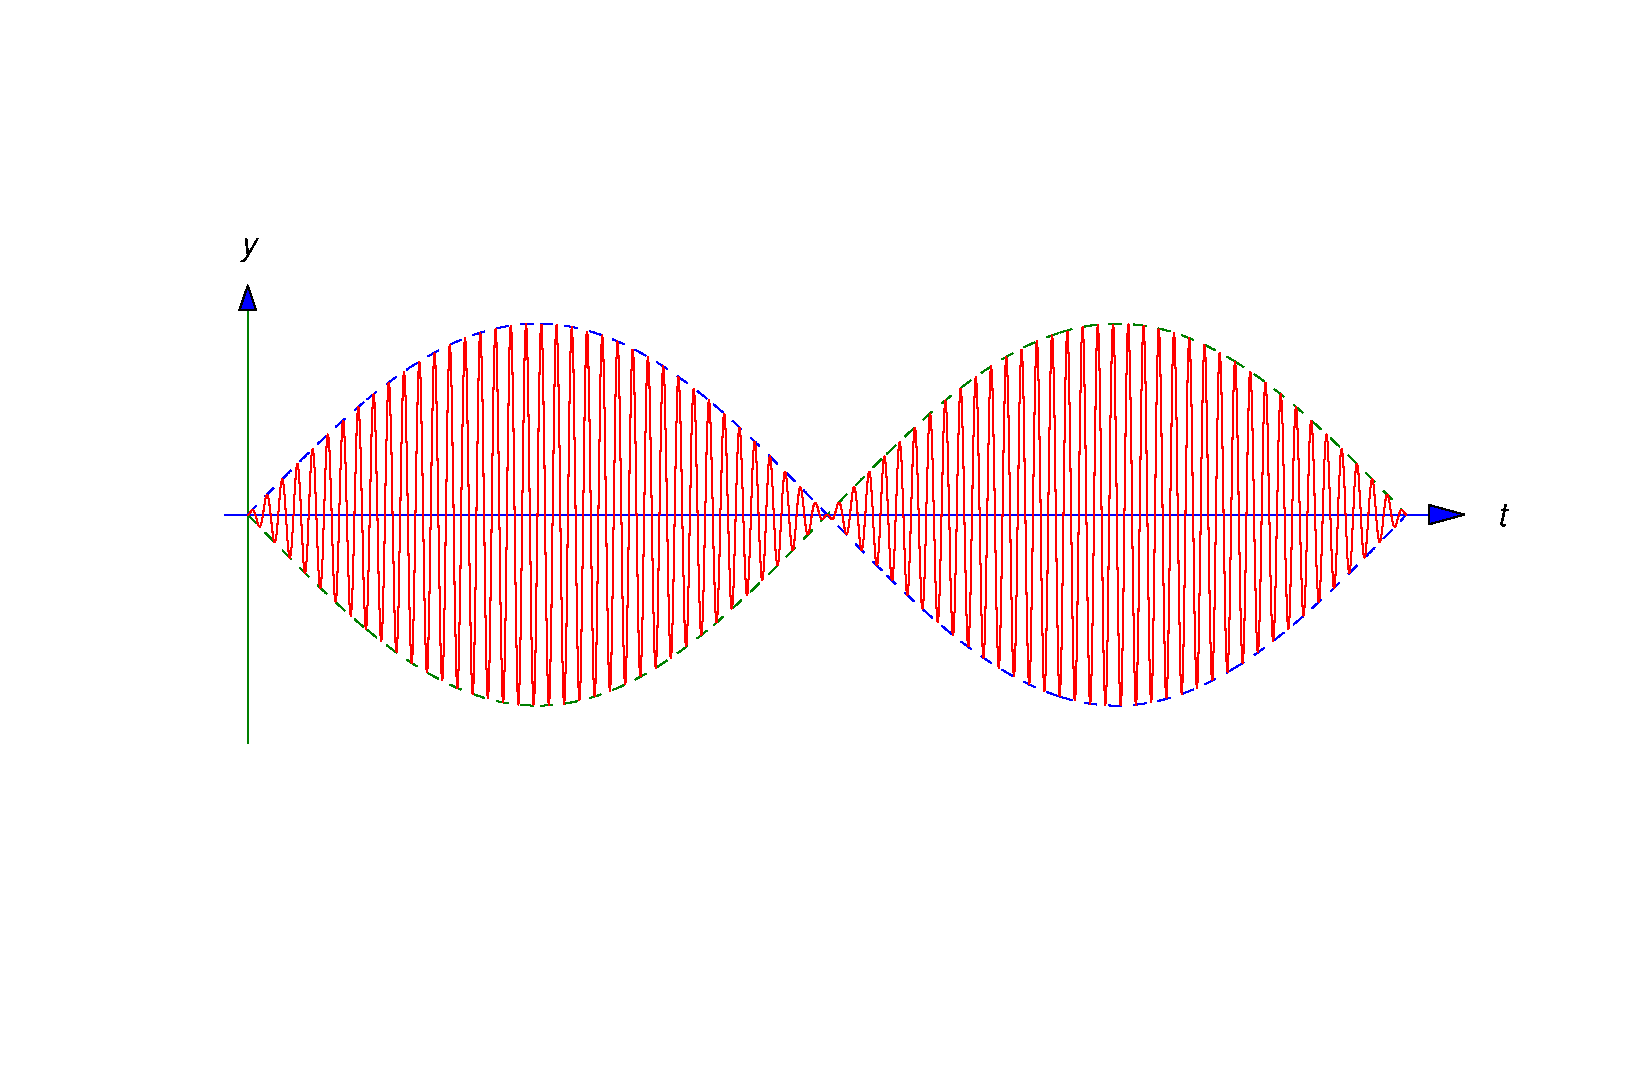
\includegraphics[bb=-78 148 689 643,width=5.67in,height=3.66in,keepaspectratio]{fig060106}
\color{blue}
\caption{ Undamped oscillation with beats}
  \label{figure:6.1.6}
\end{figure}

You can see from
\eqref{eq:6.1.20} and \eqref{eq:6.1.21} that
$$
|y(t)|\le\frac{2|F_{0}|}{m|\omega_{0}^{2}-\omega^{2}|};
$$
moreover, if $\omega+\omega_{0}$ is sufficiently large compared with $\omega
-\omega_{0}$, then $|y|$ assumes values close to (perhaps equal to) this
upper bound during each beat. However, the oscillation remains bounded for
all $t$. (This assumes that the spring can withstand
deflections of this size and continue to obey Hooke's law.)  The next
example shows that this isn't  so if $\omega=\omega_{0}$.

\begin{example}\label{example:6.1.5}\rm
Find the general solution of
\begin{equation}\label{eq:6.1.22}
y''+\omega_{0}^{2}y=\frac{F_{0}}{m}\cos\omega_{0}t.
\end{equation}
\end{example}

\solution
We first obtain a particular solution $y_{p}$ of \eqref{eq:6.1.22}. Since
$\cos\omega_{0}t$ is a solution of the complementary equation, the form
for $y_{p}$ is
\begin{equation}\label{eq:6.1.23}
y_{p}=t(A\cos\omega_{0}t+B\sin\omega_{0}t).
\end{equation}
 Then
$$
y_{p}'=A\cos\omega_{0}t+B\sin\omega_{0}t
+\omega_{0}t(-A\sin\omega_{0}t+B\cos\omega_{0}t)
$$
and
\begin{equation}\label{eq:6.1.24}
y''_{p}=2\omega_{0}(-A\sin\omega_{0}t
+B\cos\omega_{0}t)-\omega_{0}^{2}t(A\cos\omega_{0}t+B\sin\omega_{0}t).
\end{equation}
From \eqref{eq:6.1.23} and \eqref{eq:6.1.24}, we see that $y_{p}$ satisfies
\eqref{eq:6.1.22} if
$$
-2A\omega_{0}\sin\omega_{0}t+2B\omega_{0}\cos\omega_{0}t=\frac{F_{0}}{m}
\cos\omega_{0}t;
$$
that is, if
$$
A=0\mbox{\quad and \quad}B=\frac{F_{0}}{2m\omega_{0}}.
$$
Therefore
$$
y_{p}=\frac{F_{0}t}{2m\omega_{0}}\sin\omega_{0}t
$$
is a particular solution of \eqref{eq:6.1.22}. The general solution of
 \eqref{eq:6.1.22} is
$$
y=\frac{F_{0}t}{2m\omega_{0}}\sin\omega_{0}t+c_{1}\cos\omega_{0}t+c_{2}\sin\omega_{0}t.
$$
The graph of $y_{p}$ is shown in Figure~\ref{figure:6.1.7},  where it can be
seen that $y_{p}$ oscillates between the dashed lines
$$
y=\frac{F_{0}t}{2m\omega_{0}}\mbox{\quad and \quad}y=-\frac{F_{0}t}{2m\omega_{0}}
$$
with increasing amplitude that approaches $\infty$ as $t\to\infty$. Of
course, this means that the spring must eventually fail to obey Hooke's law
or break.\bbox

This phenomenon of unbounded displacements of a spring--mass system in
response to a periodic forcing function at its natural
frequency is called {\color{blue}\it resonance\/}. More complicated mechanical
structures can also exhibit resonance--like phenomena. For example,
rhythmic oscillations of a suspension bridge by wind forces or of an
airplane wing by periodic vibrations of reciprocating engines can
cause damage or even failure if the frequencies of the disturbances
are close to critical frequencies determined by the parameters of the
mechanical system in question.

\begin{figure}[tbp]
  \centering
  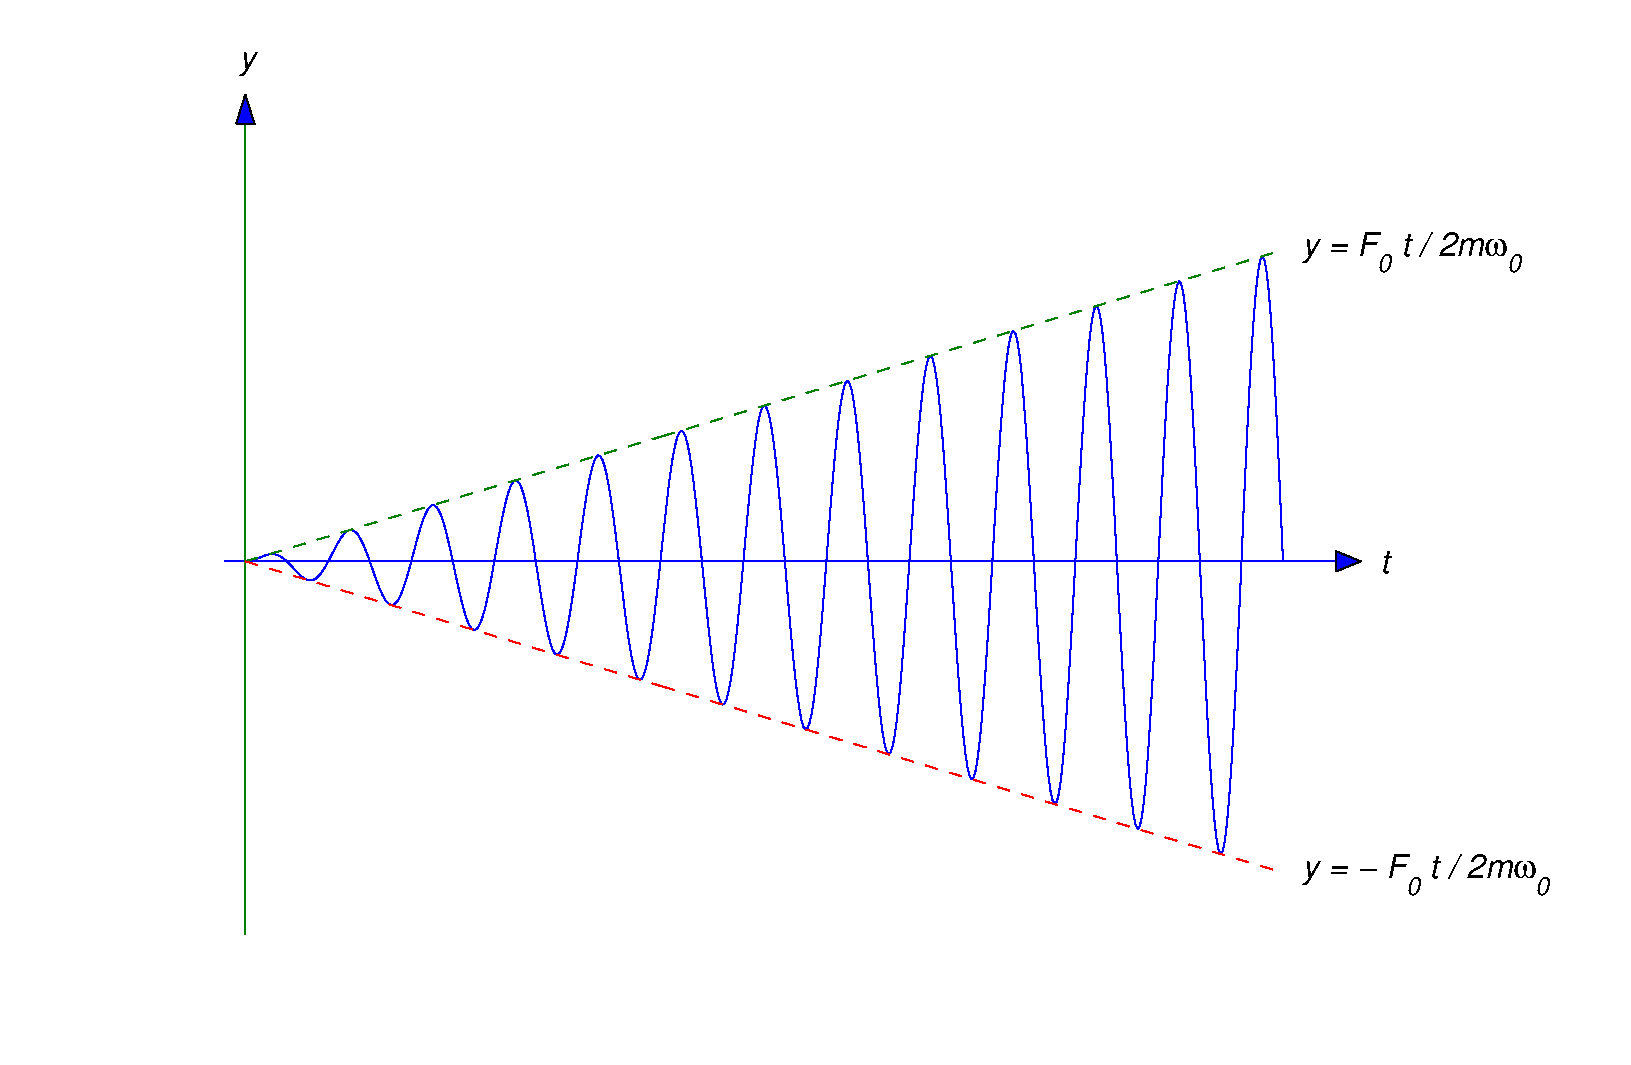
\includegraphics[bb=-78 148 689 643,width=5.67in,height=3.66in,keepaspectratio]{fig060107}
\color{blue}
\caption{ Unbounded displacement due to resonance}
  \label{figure:6.1.7}
\end{figure}

\exercises
 In the following exercises assume that there's no damping.

\begin{exerciselist}

\item\label{exer:6.1.1}   \CGex
An object stretches a spring 4 inches in equilibrium.
Find and graph its displacement for $t>0$ if it's initially displaced
36 inches above equilibrium and given a downward velocity of 2 ft/s.

\item\label{exer:6.1.2}
An object  stretches a string 1.2 inches in equilibrium.
Find its displacement for $t>0$ if it's initially displaced 3 inches
below equilibrium and given a downward velocity of 2 ft/s.

\item\label{exer:6.1.3}
A spring with natural length .5 m has length 50.5 cm with a mass of 2
gm suspended from it. The mass is initially displaced 1.5 cm below
equilibrium and released with zero velocity. Find its displacement for
$t>0$.

\item\label{exer:6.1.4}
An object stretches a spring 6 inches in equilibrium. Find its
displacement for $t>0$ if it's initially displaced 3 inches above
equilibrium and given a downward velocity of 6 inches/s. Find the
frequency, period, amplitude and phase angle of the motion.

\item\label{exer:6.1.5} \CGex
An object stretches a spring 5 cm in equilibrium. It is initially
displaced 10 cm above equilibrium and given an upward velocity of .25
m/s. Find and graph its displacement for $t>0$. Find the frequency,
period, amplitude, and phase angle of the motion.

\item\label{exer:6.1.6}
A 10 kg mass stretches a spring 70 cm in equilibrium. Suppose a 2
kg mass is
attached to the spring, initially displaced 25 cm below equilibrium,
and given an upward velocity of 2 m/s. Find its displacement for
$t>0$. Find the frequency, period, amplitude, and phase angle of the
motion.

\item\label{exer:6.1.7}
A  weight stretches a spring 1.5 inches in equilibrium. The weight
is initially displaced 8 inches above equilibrium and given a downward
velocity of 4 ft/s. Find its displacement for $t>0$.

\item\label{exer:6.1.8}
A weight stretches a spring 6 inches in equilibrium. The weight is
initially displaced 6 inches above equilibrium and given a downward
velocity of 3 ft/s. Find its displacement for $t>0$.

\item\label{exer:6.1.9}
A spring--mass system has natural frequency $7\sqrt{10}$ rad/s. The
natural length of the spring is .7 m. What is the length of the spring
when the mass is in equilibrium?

\item\label{exer:6.1.10}
A 64 lb weight is attached to a spring with constant $k=8$ lb/ft and
subjected to an external force $F(t)=2\sin t$. The weight is initially
displaced 6 inches above equilibrium and given an upward velocity of 2
ft/s. Find its displacement for $t>0$.

\item\label{exer:6.1.11}
A unit mass hangs in equilibrium from a spring with constant $k=1/16$.
Starting at $t=0$, a force $F(t)=3\sin t$ is applied to the mass. Find
its displacement for $t>0$.

\item\label{exer:6.1.12} \CGex
A 4 lb weight stretches a spring 1 ft in equilibrium. An external
force $F(t)=.25\sin8t$ lb is applied to the weight, which is
initially displaced 4 inches above equilibrium and given a downward
velocity of 1 ft/s. Find and graph its displacement for $t>0$.

\item\label{exer:6.1.13}
A 2 lb weight stretches a spring 6 inches in equilibrium.  An external
force $F(t)=\sin8t$ lb is applied to the weight, which is released
from rest 2 inches below equilibrium. Find its displacement
for $t>0$.

\item\label{exer:6.1.14}
A 10 gm mass suspended on a spring moves in simple harmonic
motion with period 4 s.  Find the period of the simple
harmonic motion of a 20 gm mass suspended from the same spring.

\item\label{exer:6.1.15}
A 6 lb weight stretches a spring 6 inches in equilibrium. Suppose
an external force $F(t)=\dst\frac{3}{16}\sin\omega
t+\dst\frac{3}{8}\cos\omega t $ lb is applied to the weight. For what
value
of $\omega$ will the displacement be unbounded? Find the displacement
if $\omega$ has this value. Assume that the motion starts from
equilibrium with zero initial velocity.

\item\label{exer:6.1.16} \CGex
A 6 lb weight stretches a spring 4 inches in equilibrium. Suppose
an external force $ F(t)=4\sin\omega t-6\cos\omega t $ lb is applied
to the weight. For what value of $\omega$ will the displacement be
unbounded? Find and graph the displacement if $\omega$ has this value.
Assume that the motion starts from equilibrium with zero initial
velocity.

\item\label{exer:6.1.17}
A mass of one kg is attached to a spring with constant $k=4$ N/m. An
external force $F(t)=-\cos\omega t-2\sin\omega t$ n is applied to the
mass. Find the displacement $y$ for $t>0$ if $\omega$ equals the
natural frequency of the spring--mass system. Assume that the
mass is initially displaced 3 m above equilibrium and given an upward
velocity of 450 cm/s.

\item\label{exer:6.1.18}
An object is in simple harmonic motion
with frequency $\omega_{0}$, with $y(0)=y_{0}$ and $y'(0)=v_{0}$. Find
its displacement for $t>0$. Also, find the amplitude of the
oscillation and give formulas for the sine and cosine of the initial
phase angle.

\item\label{exer:6.1.19}
Two objects suspended from identical springs are set into
motion.  The period of one object is twice the period of the other.
How are the weights of the two objects related?

\item\label{exer:6.1.20}
Two objects suspended from identical springs are set into motion. The
weight of one object is twice the weight of the other. How are the
periods of the resulting motions related?

\item\label{exer:6.1.21}
Two identical objects suspended from different springs are set into
motion. The period of one motion is 3 times the period of the
other. How are the two spring constants related?
\end{exerciselist}
